\documentclass[dvisvgm,tikz,border=4pt]{standalone}
\usepackage{amsmath,amssymb}

\usetikzlibrary{arrows.meta,positioning,automata,shapes,shapes.misc,calc,decorations.pathmorphing,decorations.markings,angles,quotes,patterns,mindmap,matrix,knots,hobby,trees}
\tikzset{->-/.style={decoration={markings, mark=at position 0.5 with {\arrow{Stealth}}}, postaction={decorate}}}
\begin{document}
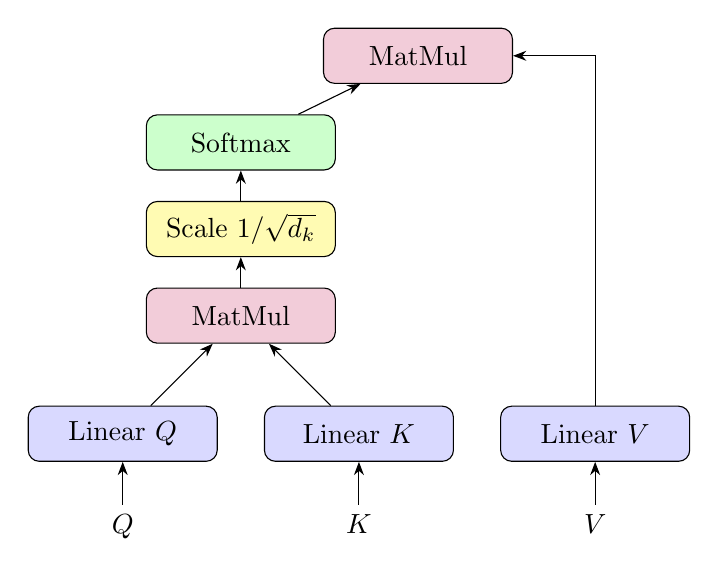
\begin{tikzpicture}[b/.style={draw, minimum width=2.4cm, minimum height=7mm, rounded corners, fill=#1}, >=Stealth]
\node[b=blue!15] (q) at (0,0) {Linear $Q$}; \node[b=blue!15] (k) at (3,0) {Linear $K$}; \node[b=blue!15] (v) at (6,0) {Linear $V$};
\node[b=purple!20] (mm) at (1.5,1.5) {MatMul}; \node[b=yellow!30] (sc) at (1.5,2.6) {Scale $1/\sqrt{d_k}$};
\node[b=green!20] (sm) at (1.5,3.7) {Softmax}; \node[b=purple!20] (mm2) at (3.75,4.8) {MatMul};
\draw[->] (q) -- (mm); \draw[->] (k) -- (mm); \draw[->] (mm) -- (sc); \draw[->] (sc) -- (sm); \draw[->] (sm) -- (mm2); \draw[->] (v) |- (mm2);
\foreach \n/\l in {q/Q, k/K, v/V} \draw[<-] (\n) -- ++(0,-0.9) node[below] {$\l$};
\end{tikzpicture}
\end{document}
